\documentclass[a4paper,10pt]{scrreprt}
	\usepackage{sty/package}
	\usepackage{sty/document}
	\usepackage{sty/math}
	\usepackage{chngcntr}
	\usepackage{mathtools}
	\usepackage{algorithm2e}
	\usepackage{enumitem}
	\usepackage{graphicx}
	\usetikzlibrary{positioning}
	\usetikzlibrary{arrows}

	\lstset{
	basicstyle=\ttfamily,
	mathescape
	}
	\setlength\parindent{0pt}
	
	\pagestyle{fancy}
	\fancyhead[R]{Cloud Computing}
	
	\counterwithout{section}{chapter}
	\counterwithin{figure}{section}
	\setcounter{chapter}{1}
	
	\renewcommand{\labelitemi}{$-$}
	
	\renewcommand*{\algorithmcfname}{Algorithmus}
	\RestyleAlgo{boxed}
	\LinesNumbered
	\SetKwInOut{Input}{Eingabe}
	\SetKwInOut{Output}{Ausgabe}

\begin{document}
	\section{Cloud Computing}
	\begin{figure}[ht]
		\centering
		
\includegraphics[width=1\textwidth]{images/cloud_computing}
	\end{figure}
	\begin{itemize}
		\item Cloud-Anbieter stellen skalierbar Hardwareressourcen zur Verfügung
		\item Software as a Service (SaaS) Anbieter stellen (darauf aufbauend) Dienste für Nutzer bereit
	\end{itemize}
	Eigenschaften von Cloud Computing Angeboten:
	\begin{itemize}
		\item Verfügbarkeit von scheinbar unbegrenzten Ressourcen
		\item Keine Kapazitätsplanung aus Sicht des Nutzers mehr nötig
		\item Pay-as-you-go Modell\\[5pt]
			$\hookrightarrow$ Kosten werden durch die tatsächliche Nutzung bestimmt
	\end{itemize}
	Resultat:
	\begin{itemize}
		\item economic of scale\\[5pt]
		$\hookrightarrow$ Geringere Anschaffungs- und Betriebskosten\\[5pt]
		$\hookrightarrow$ Höhere Auslastung als konventionelle Datenzentren
		\item Nutzer sparen Kosten und reduzieren finanzielle Risiken\\[5pt]
		$\hookrightarrow$ keine/wenig Hardware Anschaffung\\[5pt]
		$\hookrightarrow$ Bedarf wird nicht unter- oder überschätzt\\[5pt]
		$\hookrightarrow$ Neue Angebote können schneller auf den Markt gebracht werden
	\end{itemize}
	\subsection{Basistechnologien}
	\subsubsection{Virtualisierung}
	\begin{itemize}
		\item Kann auf verschiedenen Ebenen erfolgen (z.B. Betriebssysteminstanz)
		\item Bessere Ausnutzung von Hardwareressourcen\\[5pt]
		$\hookrightarrow$ Ermöglicht mehrere Benutzer auf einer physischen Maschine\\[5pt]
		$\hookrightarrow$ Entkoppelung von Ausführungsort und Hardware 
		\item Isolation von Nutzern
	\end{itemize}
	\subsubsection{Web-Services}
	\begin{itemize}
		\item Sprachunabhängige Basis für entfernte Kommunikation/Interaktion
	\end{itemize}
	\subsection{Cloud Computing - Erweiterte Architektur}
	\subsubsection{Software as a Service (SaaS)}
	\begin{itemize}
		\item Vom Endnutzer oder anderen SaaS Einheiten genutzte Dienste
	\end{itemize}
	\subsubsection{Function as a Service (FaaS)}
	\begin{itemize}
		\item Ausführungsumgebung für einzelne Funktionen
	\end{itemize}
	\subsubsection{Platform as a Service (PaaS)}
	\begin{itemize}
		\item Konfektionierte Middleware für skalierbare Anwendungen
	\end{itemize}
	\subsubsection{Infrastructure as a Service (IaaS)}
	\begin{itemize}
		\item Mittels Virtualisierung bereitgestellte Ressourcen
	\end{itemize}
	\subsection{Einsatzszenarien}
		\subsubsection{Public Cloud}
	\begin{itemize}
		\item Mieten von entfernten Ressourcen
	\end{itemize}
	\subsubsection{Private Cloud}
	\begin{itemize}
		\item Durch Virtualisierung flexibilisierte Verwaltung von Ressourcen
		\item Oder durch zusätzliche Mechanismen geschaffene Infrastruktur für einen Nutzer (z.B. Innerhalb von Amazon EC2)
	\end{itemize}
	\subsubsection{Hyprides Cloud Computing}
	\begin{itemize}
		\item Eigene Ressourcen mit denen einer öffentlichen Cloud kombinieren
		\item IT Infrastruktur schon vorhanden
		\item Kritische Daten, die nicht ausgelagert werden können
		\item Öffentliche Cloud nur zur Deckung von Bedarfsspitzen
	\end{itemize}
	\subsubsection{Multi-cloud Computing}
	\begin{itemize}
		\item Parallele Verwendung verschiedener Anbieter
	\end{itemize}
	\section{Virtualisierung}
	Die Infrastruktur zur Virtualisierung wird \textbf{Virtual Machine Monitor (VMM)} oder \textbf{Hypervisor} genannt, die virtuelle Plattform entsprechend \textbf{Virtual Machine (VM)}.
	\begin{figure}[ht]
		\centering
		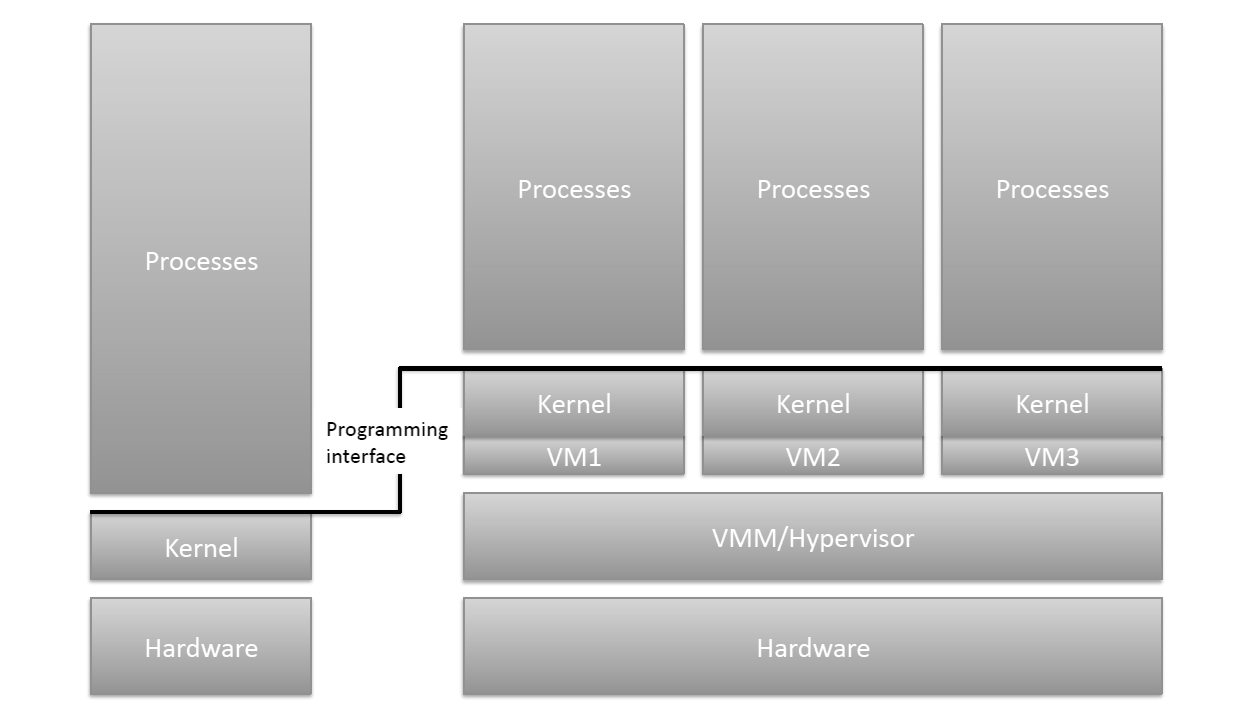
\includegraphics[width=1\textwidth]{images/virtualisierung}
	\end{figure}\\
	Für eine virtuelle Maschine gelten folgende Bedingungen:
	\begin{itemize}
		\item \textbf{Äquivalenz}\\[5pt]
		$\hookrightarrow$ Ein Programm verhält sich äquivalent zur direkten Ausführung\\[5pt]
		$\hookrightarrow$ Tolerierte Abweichungen sind geringere Verfügbarkeit an Ressourcen und \hspace*{12pt} geändertes zeitliches Verhalten 
		\item \textbf{Isolation}\\[5pt]
		$\hookrightarrow$ VMs, die zusammen auf einer realen Plattform laufen, sollen effektiv vonein-\hspace*{14pt}ander isoliert sein\\[5pt]
		$\hookrightarrow$ VMM hat die komplette Kontrolle über die Hardwareressourcen\\[5pt]
		$\hookrightarrow$ VMs können nicht auf Ressourcen zugreifen, die ihnen nicht zugewiesen wur-\hspace*{14pt}den\\[5pt]
		$\hookrightarrow$ VMM kann unter bestimmten Umständen die Kontrolle über zugewiesene \hspace*{12pt} Ressourcen wieder entziehen
		\item\textbf{Effizienz}\\[5pt]
		$\hookrightarrow$ Der weitaus größere Teil an Instruktionen des virtuellen Prozessors muss \hspace*{12pt} direkt ohne Interaktion des VMMs, auf dem realen Prozessor ausgeführt \hspace*{13pt} werden
	\end{itemize}
	Letzte Anforderung ist nicht zwingen notwendig.
	\subsection{Ziele von Virtualisierung}
	\begin{itemize}
		\item Bessere Ausnutzung existierender Ressourcen
		\item Erhöhung von Verlässlichkeit und Sicherheit
		\item Höhere Skalierbarkeit von Systemen
		\item Zentralisierung von Altsystemen ohne alte Hardware
	\end{itemize}
	\subsection{Kritische Punkte bei der Virtualisierung}
	\begin{itemize}
		\item Ausführung durch die CPU\\[5pt]
		$\hookrightarrow$ VMM emuliert eine CPU bzw. stellt eine virtuelle CPU zur Verfügung
		\item Zugriff auf Speicher mittels der MMU\\[5pt]
		$\hookrightarrow$ VMM muss den virtuellen Speicher emulieren (oder durch HW)
		\item Beim Zugriff auf Geräte werden Interrupts verwendet\\[5pt]
		$\hookrightarrow$ VMM muss Interrupts an Geräte weiterleiten
		\item Reaktion von Endgeräten (I/O) wird in Form von Interrupts vermittelt\\[5pt]
		$\hookrightarrow$ VMM muss die Interrupts in das System weiterleiten
		\item Zugriff auf Betriebssystem-Elemente unter Verwendung von Traps\\[5pt]
		$\hookrightarrow$ VMM muss Software-Interrupts an die entsprechende Stelle weiterleiten und \hspace*{12pt} die Verwaltung von Interrupt Tabellen virtuell gestalten
		\item Exceptions müssen behandelt werden können
	\end{itemize}
\newpage
	\subsection{Ebenen der Virtualisierung}
	\subsubsection{Instruction Set Architecture (ISA) bzw. Interface}
	\begin{itemize}
		\item Schnittstelle der Hardware zum Betriebssystem und zu den Anwendungen
		\item System-virtuelle Maschinen virtualisieren das ISA
	\end{itemize}
	\subsubsection{Application Binary Interfce (ABI)}
	\begin{itemize}
		\item Schnittstelle zum Betriebssystem, die Applikationen bzw. Prozesse nutzen
		\item Prozess-virtuelle Maschinen virtualisieren das ABI
	\end{itemize}
	\begin{figure}[ht]
		\centering
		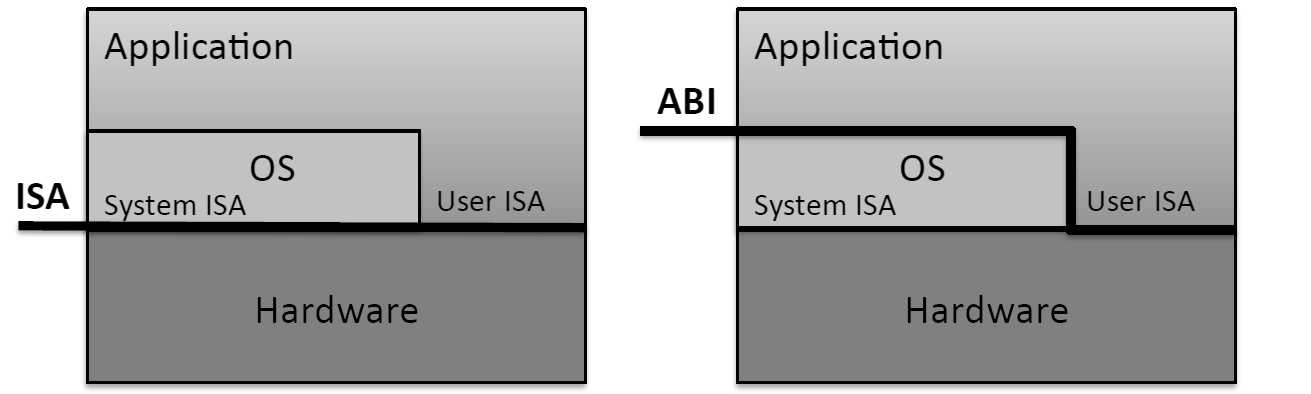
\includegraphics[width=.8\textwidth]{images/isa_abi}
	\end{figure}
	\subsection{System Virtualisierung}
	\subsubsection{Vollständige Virtualisierung}
	\begin{itemize}
		\item Keine Anpassung des Gastsystems nötig
		\item Unterstützung von fremder HW\\[5pt]
		$\hookrightarrow$ emuliert ISA auf fremder HW
		\item Beispiele: VMware Workstation, QEMU, Bochs
	\end{itemize}
	\begin{figure}[ht]
		\centering
		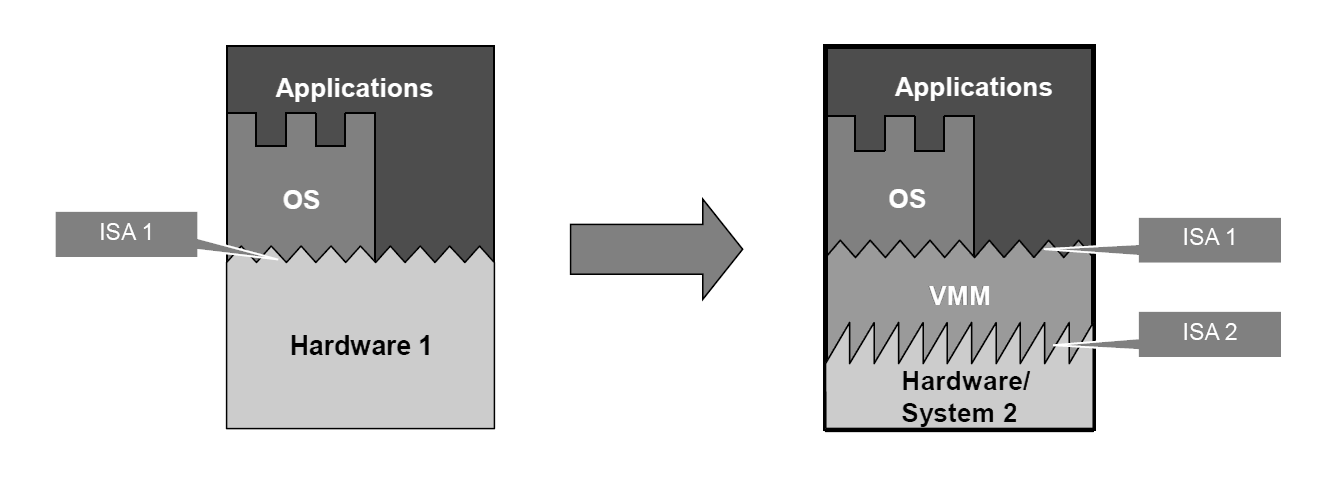
\includegraphics[width=1\textwidth]{images/vollstaendige}
	\end{figure}
	\subsubsection{Hybrid Betrieb}
	\begin{itemize}
		\item Beispiel: Linux läuft nativ und Windows wird in einer virtuellen Maschine ausgeführt
	\end{itemize}
	\begin{figure}[ht]
		\centering
		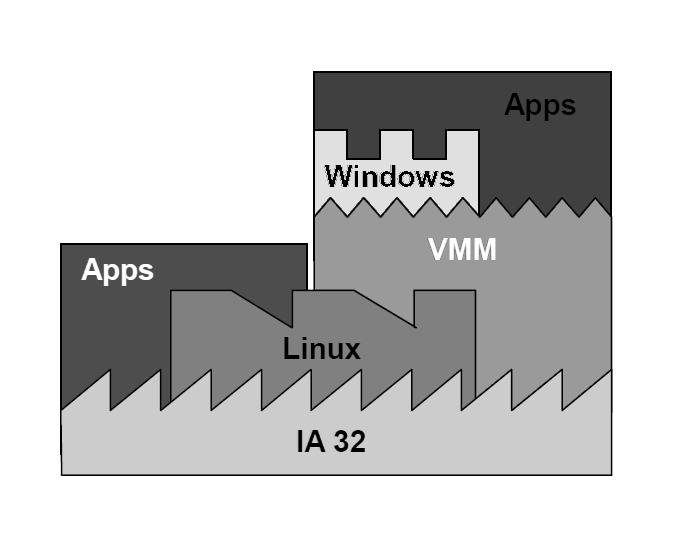
\includegraphics[width=0.5\textwidth]{images/hybrid}
	\end{figure}
	\subsubsection{Hardware-basierte Virtualisierung}
	\begin{itemize}
		\item Wenn die gleiche ISA virtualisiert wird kann zur Optimierung die ISA direkt verwendet werden\\[5pt]
		$\hookrightarrow$ Beispiele: VMware (Linux/Windows auf x86)
		\item Voraussetzung: Hardware-Unterstützung von Virtualisierung bzw. Schutz gewisser Einheiten durch VM\\[5pt]
		$\hookrightarrow$ Beispiele: Intel VMM/VMX
		\begin{itemize}
			\item VMX-Instruktionen zum Generieren und Kontrollieren einer virtuellen Umgebung
			\item VMM kontrolliert Interrupts und Exceptions
			\item Memory Virtualisierung
		\end{itemize}
	\end{itemize}
	\begin{figure}[ht]
		\centering
		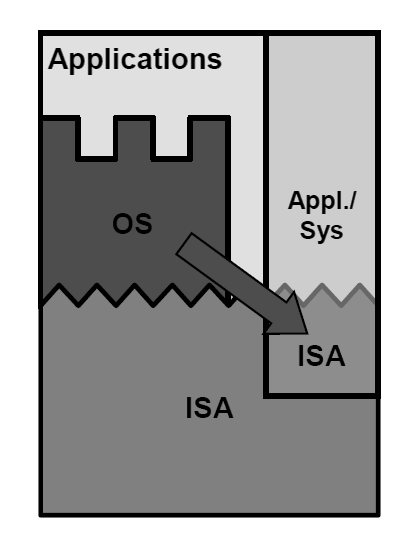
\includegraphics[width=0.3\textwidth]{images/hardware}
	\end{figure}
\newpage
	\subsubsection{Paravirtualisierung}
	\begin{itemize}
		\item Trennung von Host- und Gastbetriebssystem
		\item Gastbetriebssystem muss definierte Schnittstellen implementieren\\[5pt]
		$\hookrightarrow$ Erleichtert Kontrolle des Gastsystems\\[5pt]
		$\hookrightarrow$ Direkter Zugriff auf Hardware kann verhindert werden
	\end{itemize}
	\begin{figure}[ht]
		\centering
		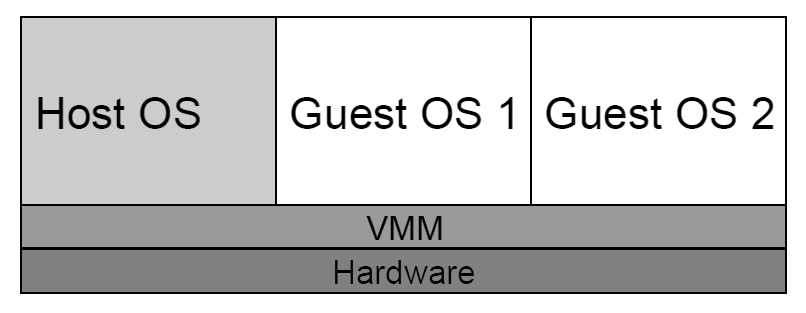
\includegraphics[width=0.6\textwidth]{images/para}
	\end{figure}
	\subsection{Virtualisierung auf Ebene der ABI}
	\begin{itemize}
		\item Stellt unifizierte Laufzeitumgebung unter evtl. verschiedenen Betriebssystemen zur Verfügung
		\item Beispiele: Betriebssystem-Virtualisierung (z.B. Docker), WINE und High Level Language Virtual Machines
	\end{itemize}
	\begin{figure}[ht]
		\centering
		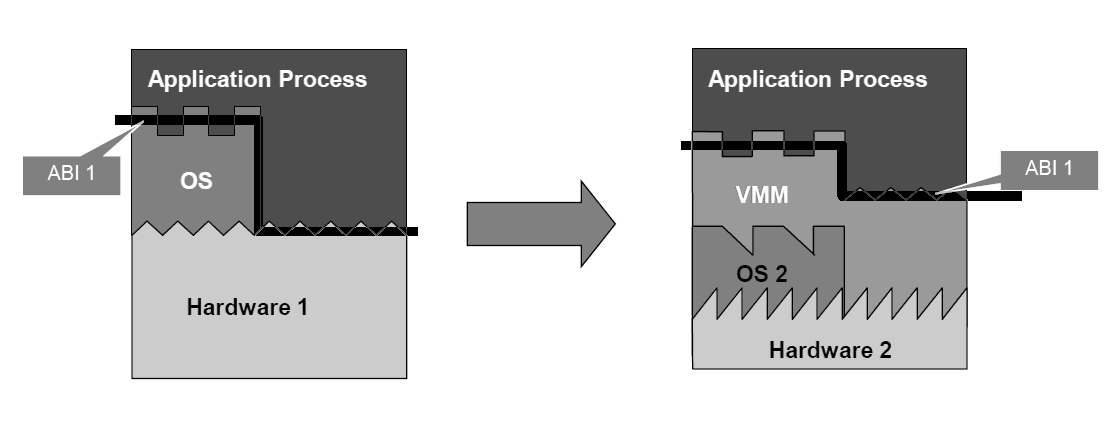
\includegraphics[width=1\textwidth]{images/v_abi}
	\end{figure}
\newpage
	\subsubsection{Betriebssystem-Virtualisierung}
	\begin{itemize}
		\item Oft werden mehrere Betriebssystem-Instanzen inklusive des gleichen Kernels verwendet um verschiedene Dienste bereitzustellen
		\item Um Ressourcen zu sparen und hohe Effizienz zu erlangen ermöglicht Betriebssystem-Virtualisierung die gemeinsame Nutzung eines Kernels und dennoch eine isolierte Ausführung
		\item Verwendung des gleichen Kernels erfordert nur sehr geringe Kontextanpassungen und kann entsprechend hohe Performanz bieten
		\item Beispiel; VServer - aktuell: Docker
	\end{itemize}
	Anforderungen:
	\begin{itemize}
		\item Einsatz von Mechanismen zur Umsetzung von Ressource- und Sicherheitscontainern für Isolation
	\end{itemize}
	\begin{figure}[ht]
		\centering
		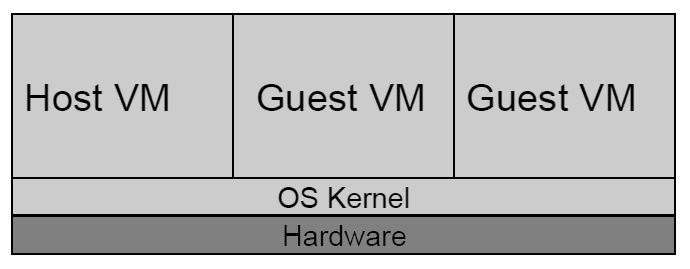
\includegraphics[width=.6\textwidth]{images/betriebssystem}
	\end{figure}
\newpage
	\subsubsection{High Level Language (HLL) VMs}
	\begin{itemize}
		\item Virtualisiert (in der Regel) keine reale Maschine
		\item Entwurf gemeinsam mit der Applikationsumgebung für die HLL
		\item Vorteile: Portabilität, zugeschnitten auf HLL
		\item Wird aktuell relevanter im Kontext Cloud Computing durch FaaS
		\item Beispiele: Java VM, JavaScript, .NET CLI
	\end{itemize}
	\begin{figure}[ht]
		\centering
		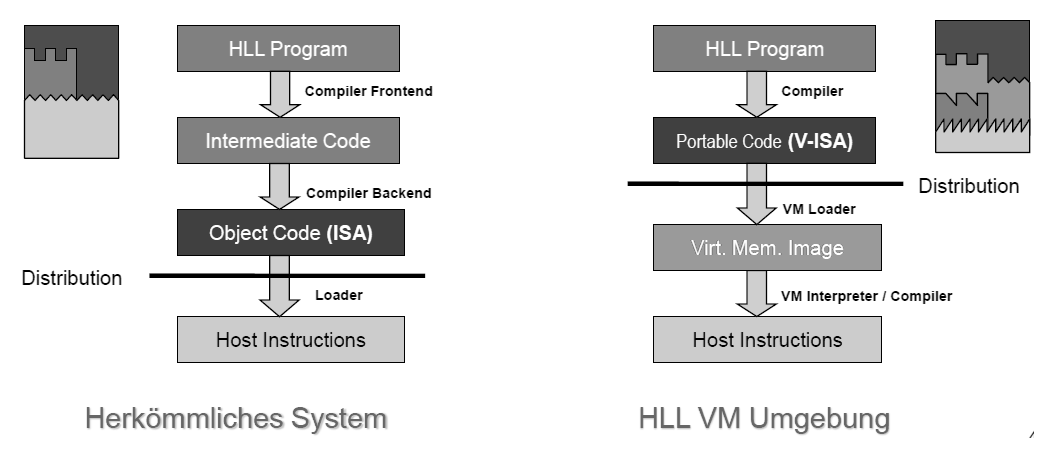
\includegraphics[width=1\textwidth]{images/hll}
	\end{figure}
	\subsection{Aufbaue einer virtuellen Maschine}
	\begin{itemize}
		\item Notwendige Betriebsmittel
		\begin{itemize}
			\item Physische Maschine und Gastgeberbetriebssystem (Host)
			\item Virtualisierungssoftware, die den VMM bereitstellt
			\item Abbild der zu betreibenden virtuellen Maschine
		\end{itemize}
		\item Ausbau des Abbilds einer virtuellen Maschine
		\begin{itemize}
			\item Meta-Informationen (spezifisch, je nach Virtualisierungssoftware)
			\item Dateisystem
			\begin{itemize}
				\item Kern des zu virtualisierenden Gastbetriebssystem (Guest)
				\item User-Space-Komponenten des Gastbetriebssystems
				\item Daten
			\end{itemize}
		\end{itemize}
	\end{itemize}
	Analogie Objektorientierung:
	\begin{itemize}
		\item Klasse: statisches Abbild einer VM
		\item Instanz: eine im Betrieb befindliche VM
	\end{itemize}
\newpage
	\section{Infrastructure as a Service}
	\begin{figure}[ht]
		\centering
		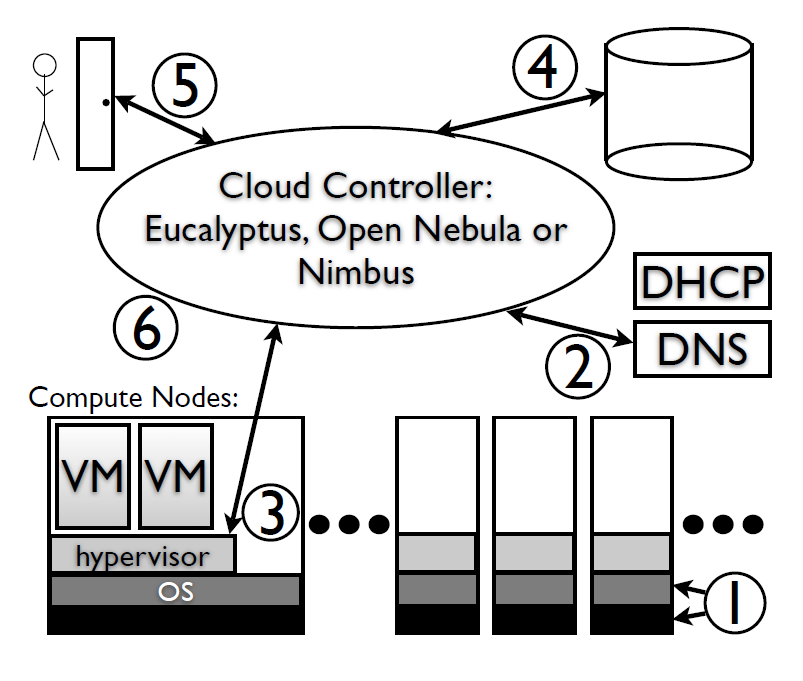
\includegraphics[width=.7\textwidth]{images/iaas}
	\end{figure}
	\begin{enumerate}
		\item Hardware und Betriebssystem
		\item Netzwerk und Netzwerkdienste (z.B. DHCP, DNS)
		\item Virtualisierung
		\item Datenspeicher und Image-Verwaltung
		\item Managementschnittstelle für Administratoren und Benutzer
		\item Cloud-Controller\\[5pt]
		$\hookrightarrow$ Management der Ressourcen
	\end{enumerate}
	\subsubsection{Netzwerk und Netzwerkdienste}
	\begin{itemize}
		\item Verwaltung und Einbindung der realen und der virtuellen Infrastruktur
		\item Zuordnung einer eindeutigen (virtuellen) MAC pro virtueller Maschine
		\item Vermittlung des Datenverkehrs zwischen der realen Maschine und den virtuellen Maschinen (bridge)
		\item Automatische Einbindung mittels DHCP (Zuordnung einer IP-Adresse) und DNS (Zuordnung eines Host-Namens)
		\item Eventuell Etablierung privater Netzwerke etc.
	\end{itemize}
	Umsetzung:
	\begin{itemize}
		\item Cloud-Controller muss bei Erzeugung einer virtuellen Maschine die Virtualisierungsinfrastruktur konfigurieren und entsprechende Informationen an den DHCP- sowie DNS-Server weitergeben
	\end{itemize}
	\subsubsection{Virtualisierung}
	\begin{itemize}
		\item Xen, KVM, VServer, etc.
		\item Im Open-Source-Bereich wird oft von der verwendeten Virtualisierungslösung mittels libvirt abstrahiert
	\end{itemize}
	Umsetzung libvirt:
	\begin{itemize}
		\item Stellt einheitliche Schnittstelle zum Verwalten von unterschiedlichen Virtualisierungslösungen zur Verfügung
		\item Einfache C-Schnittstelle und Kommandozeilenunterstützung\\[5pt]
		$\hookrightarrow$ z.B. Starten, Stoppen, Migrieren und Pausieren von VMs
		\item Kommandos werden über libvirtd entgegengenommen\\[5pt]
		$\hookrightarrow$ Ermöglicht lokales wie auch entferntes Management von VMs
	\end{itemize}
	\begin{figure}[ht]
		\centering
		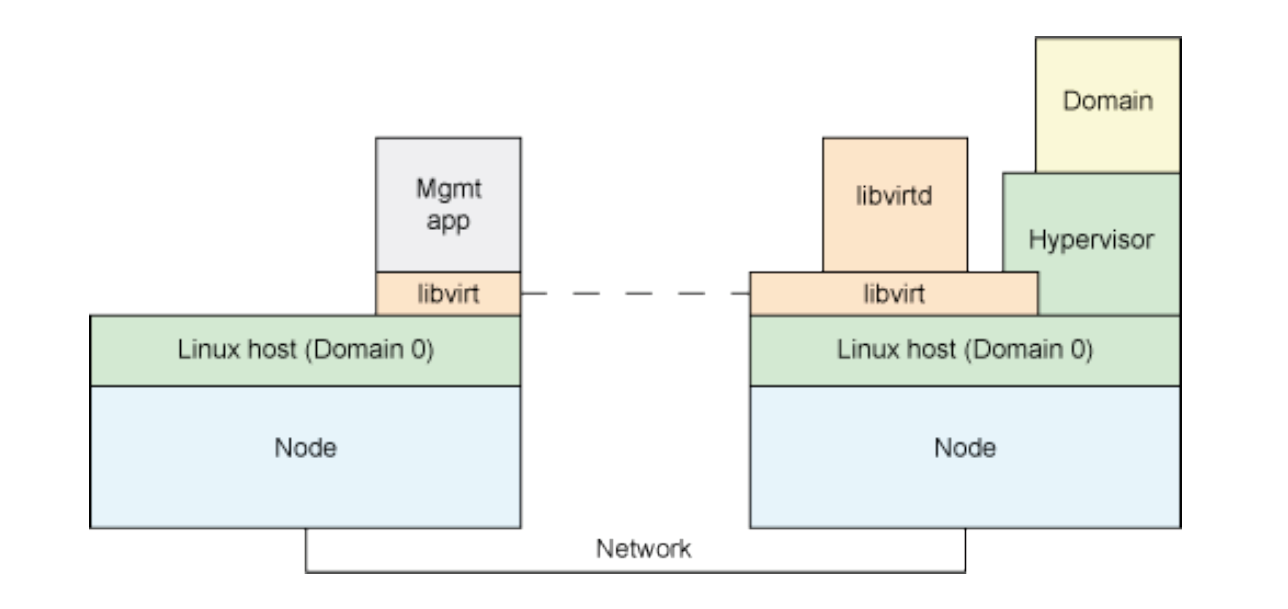
\includegraphics[width=.9\textwidth]{images/libvirt}
	\end{figure}
	\subsubsection{Datenspeicher und Image-Verwaltung}
	\begin{itemize}
		\item Schnelle Erzeugung und De-/Installation von VM-Images\\[5pt]
		$\hookrightarrow$ Images müssen konfiguriert und eventuell um spezifische Software ergänzt \hspace*{12pt} werden
	\end{itemize}
	Umsetzung:
	\begin{itemize}
		\item Repository für VM-Images\\[5pt]
		$\hookrightarrow$ In der Regel Vorlagen, die erst noch in ein lauffähiges System umgewandelt \hspace*{12pt} werden (z.B. durch hinzufügen einer Swap-Partition oder Anpassung der \hspace*{12pt} Partitionsgröße)
	\end{itemize}
	\subsubsection{Managementschnittstelle für Benutzer}
	\begin{itemize}
		\item In der Regel grafische Benutzeroberfläche für den Anwender
		\begin{itemize}
			\item Anfordern neuer VMs
			\item Benutzerspezifische Konfiguration\\[5pt]
			$\hookrightarrow$ z.B. Amazon EC2: Größenklassen für VMs oder Ort der Ausführung
			\item Verwaltung von Credentials für den sicheren Zugriff auf VMs
		\end{itemize}
	\end{itemize}
	\subsubsection{Cloud-Controller}
	\begin{itemize}
		\item Zentrale Komponente einer IaaS-Infrastruktur
		\item Umsetzung der Benutzeranforderungen für die Erzeugung von VM-Images und ihre Installation
		\item Um-/Verteilung von VMs
	\end{itemize}
\newpage
	\section{Datenmanagement in Clouds}
	\begin{itemize}
		\item Allgemeiner Trend: Extreme Zunahme der zu verarbeitenden Daten\\[5pt]
		$\hookrightarrow$ Induziert durch Zunahme an computergestützter Datenverarbeitung und ex-\hspace*{12pt} ponentieller Zunahme der Kapazität von Speichermedien bei gleichen Kosten
		\item Problematik: Effiziente und skalierbare Verarbeitung von Daten
		\item Lösungsansatz: Neue Konzepte bzw. Algorithmen für verteiltes Datenmanagement
		\item Programmiermodell: MapReduce/Hadoop, Dryad
		\item Verteilte, einfache Datenbank-ähnliche Systeme bzw. Key-Value-Stores: Dynamo, BigTable, PNUTS
		\item Verteilte Dateisysteme: GoogleFS, HadoopFS
	\end{itemize}
\newpage
	\section{Web-Service}
	\begin{itemize}
		\item Zentraler Begriff der Dienstleistung\\[5pt]
		$\hookrightarrow$ Komponente bietet Dienst an
		\item Zugang zu Web-Services über das Web\\[5pt]
		$\hookrightarrow$ Nutzung standardisierter Protokolle und Konzepte
	\end{itemize}
	\begin{itemize}
		\item Vision vom Markt der Komponenten (Web-Services)\\[5pt]
		$\hookrightarrow$ Unabhängige Softwarefirmen verkaufen Web-Services-Software\\[5pt]
		$\hookrightarrow$ Web-Services sind nicht ortsgebunden\\[5pt]
		\hspace*{20pt}$\hookrightarrow$ Kann aus der Entfernung zugegriffen werden\\[5pt]
		\hspace*{20pt}$\hookrightarrow$ Benötigt in der Regel keine Installation von Software für den Nutzer
		\item Web als einfache Schnittstelle
	\end{itemize}
	\subsubsection{Definition Web-Services}
	Ein Dienst, dessen Schnittstelle mit \textbf{WSDL} beschrieben, mit \textbf{UDDI} registriert und gefunden und mit \textbf{SOAP} angesprochen werden kann.
\end{document}
